%****************************************************
%	CHAPTER 2 - Prototype Design
%****************************************************
\chapter{Prototype Design}
\label{ch:proto}
%====================================================
\section{Conventions Used}
\label{sec:proto.conventions}
Attitude conventions used for the plants' dynamic derivations in the following Chapter:\ref{ch:dynamics} are briefly discussed here. Often these aspects are omitted or assumed to be known already, it's important to clearly and unambiguously define a standard set frames to avoid uncertainty in the kinematics. Rotation matrices and angles are included briefly for the sake of completeness but the focus is on \emph{contrast} between rotation and transformation operations. Both \cite{spacecraftattitutdequaternions} and \cite{rigidbodylecture} provide an in depth and thorough explanation of rotational matrices and DCM attitude representation if such concepts are unfamiliar to the reader.
%====================================================
\subsection{Reference Frames Convention}
\label{subsec:proto.conventions.frames}
%====================================================
\begin{figure}[htbp]
\centering
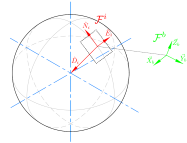
\includegraphics[width=0.6\textwidth]{figs/reference_frame}
\caption{Inertial and Body Reference Frames}
\label{fig:ref_frame}
\end{figure}
Regular aerospace (Euler) frames are used for principle inertial and body directions. Shown in Fig: \ref{fig:ref_frame}, the inertial frame,~$\mathcal{F}^i$, is aligned such that the $\vec{X}_i$ axis is in the $\hat{N}$orth direction, $\vec{Y}_i$ is in the $\hat{E}$ast direction and $\vec{Z}_i$ is  in the $\hat{D}$ownward direction\footnote{In orbital sequences this would be toward the Earths' center. Sometimes referred to as the NED convention}. The body frame, $\mathcal{F}^b$, then has both $\vec{X}_b$ and $\vec{Y}_b$ aligned with two perpendicular arms of the quadrotors' body and finally the $\vec{Z}_b$ axis pointing in the body's normal direction. The body frames' axes and their relation to the prototype design are highlighted next in Sec:\ref{subsec:proto.conventions.motoraxis}. Frame superscripts $i$ and $b$ represent inertial and body frames respectively. Vector subscripts imply the reference frame in which the vectors' coordinates exists in. 
\par
The relative angular displacement between the two frames is commonly measured by the three angle Euler set. The Euler set $[\psi ~\theta ~\psi]^T$ represents rotations about the $\vec{X}$,$\vec{Y}$ and $\vec{Z}$ axes respectively. Depending on how the rotation sequence is formulated, those angles can be used to construct rotation matrices which give relation to vectors or can transform coordinates. The generic equation for a rotation of a vector $\vec{v}$ about a (normalized) axis $\hat{n}$ by some angle $\mu$ is given by\footnote{Derived in \cite{quaddynamics}}:
\begin{equation}\label{eq:genrotationmatrix}
\vec{v}~'=\big(1-cos(\mu)\big)\big(\vec{v}\cdot \hat{n}\big)\hat{n}+cos(\mu)\vec{v}+sin(\mu)\big(\hat{n}\times\vec{v}\big)
\end{equation}
Which, when $\hat{n}$ is either $\vec{X}$,$\vec{Y}$ or $\vec{Z}$ axes, can be simplified to produce the common rotation matrices $\mathbb{R}_x(\psi)$,$\mathbb{R}_y(\theta)$ and $\mathbb{R}_z(\phi)$. Multiplication by a rotation matrix $\mathbb{R}(\cdot)$ applies a \emph{rotation} operator, the output vector still exists in the same reference frame, for a vector $\vec{v}\in\mathcal{F}^i$;
\begin{subequations}
\begin{equation}\label{eq:rotationoperator.a}
\vec{v}~'=\mathbb{R}_{x}(\psi)\vec{v}
\end{equation}
\vspace{-20pt}
\begin{equation}\label{eq:rotationoperator.b}
\vec{v}~',\vec{v}\in\mathcal{F}^i
\end{equation}
\end{subequations}
A \emph{transformation} changes the vectors reference frame. The transformation is a rotation by a transformation angle which is difference between the resulting reference frame and the principle reference frame. A transformation from frame $\mathcal{F}^i$ to $\mathcal{F}^b$ by an angle of $\psi$ about the $\vec{X}$ axis then produces  

$\mathbb{R}_{x}(\psi)$ is a rotation by $\psi$ and $\mathbb{R}_{x}(-\psi)$ is a transformation.


A rotation matrix $\mathbb{R}_{x}(\psi)$ represents a rotation around the $\vec{X}$ axis by $\psi$ radians and can similarly be extrapolated for other axes.
Vectors are rotated by a multiplication operation, for a vector, $\vec{v}$, in a given reference frame $i$(not necessarily the inertial frame) it follows that:
\begin{subequations}
\begin{equation}\label{eq:rotationmatrix}
\vec{v}\in\mathcal{F}^i
\end{equation}
\vspace{-20pt}
\begin{equation}
\vec{v}^{'}=\mathbb{R}_{x}(\psi)\times\vec{v}
\end{equation}
\end{subequations}
\par
An inherent singularity does exists with such attitude representations. Indeed Quaternions are used later in Sec: \ref{subsec:dynamics.rigidbody.quaternion} in lieu of Euler angles, but they are easily understood and well suited to illustrate the distinction between rotation and transformation angles made here.
\par

\subsection{Motor Axis Layout}
\label{subsec:proto.conventions.motoraxis}
%****************************************************

%****************************************************
\section{Design}
\label{sec:proto.design}
%****************************************************
\subsection{Gimbal Articulation}
\label{subsec:proto.design.actuation}
%****************************************************
\subsection{Inertial Matrix Function}
\label{subsec:proto.design.inertia}
%****************************************************
\subsection{Overall Aspects}
\label{subsec:proto.design.aspects}
%****************************************************
\subsubsection{Vibration Damping}
%****************************************************
\subsubsection{Duct}
%****************************************************
\subsubsection{Landing Skids}
%****************************************************
\subsubsection{Motors \& ESCs}
%****************************************************

%****************************************************
\section{System Layout}
\label{sec:proto.layout}
%****************************************************
